\documentclass[11pt, a4paper]{article}
\usepackage[english, science, small]{ku-frontpage}
\usepackage[utf8]{inputenc}
\usepackage[cache=false]{minted}
\usepackage{caption}

% Math stuff
\usepackage{amsmath,amssymb,mathtools,bm,etoolbox,stmaryrd}
% verctor command. Usage: \colvec{5}{a}{b}{c}{d}{e}
\newcount\colveccount
\newcommand*\colvec[1]{
	\global\colveccount#1
	\begin{pmatrix}
		\colvecnext
	}
	\def\colvecnext#1{
		#1
		\global\advance\colveccount-1
		\ifnum\colveccount>0
		\\
		\expandafter\colvecnext
		\else
	\end{pmatrix}
	\fi
}

% que dymbol, textmode
\newcommand*{\qed}{\hfill\ensuremath{\square}}%

% TOC properties
\setlength\arraycolsep{2 pt}
\setcounter{tocdepth}{2}
\setcounter{secnumdepth}{2}

\author{Per Steffen Czolbe (wjq874)}
\title{Reinforcement Learning with LEGO Mindstorms}
\subtitle{Project Report}
\date{Handed in: \today}

\begin{document}
\maketitle

\section{Abstract}

\tableofcontents


\section{Introduction}
scientific goal,
educational goals,
agenda by lego

\subsection{The ev3 robot}

\subsubsection{Hardware}
central component: the "brick"
cpu: 32bit, 300MHz ARM9 Processor
Memory: 64MB DDR RAM
Storage: 16MB Flash
up to 32gb SD-card

Communication:
USB
Bluetooth
wifi

Periferals:
up to 4 motors and 4 sensors.

src: LEGO MINDSTORMS EV3 Hardware Developer Kit (pdf) ©2013 The LEGO Group


\subsubsection{Default Software}
The ev3 is shipped with LEGOs own graphical programming software, based on the visual programming language LabVIEW.

Many community driven software packages exist. These support languages such as matlab, python, java, javascript, C++, C, GO, Ruby, Perl, R, Lue and may more (src: https://www.ev3dev.org/docs/programming-languages/). Direct control of the robot via command line is also possible.



\section{Development Setup}
- tutorial style description of how to get things to run with jupyter notebook.

\subsection{New software: ev3dev}
"ev3dev is a Debian Linux-based operating system that runs on several LEGO® MINDSTORMS compatible platforms including the LEGO® MINDSTORMS EV3 and Raspberry Pi-powered BrickPi." src: https://www.ev3dev.org/

Because of the limited storage available on the Brick, this ~2GB linux image has to be added to the ev3 via an SD-Card.

\subsection{External Computer for computations}
While the brick runs a fully fletched linux system that can execute programms on it's own, the processing and memory contraints of the brick limit development of programms severely. Installing a new python package with pip often takes over 2 minutes. Installing deep learning frameworks like tensorflow, or performing image processing on the brick is expected to lead to severe sortages of processing power. Thus we want to run these more computationally expensive parts of the program on a seperate computer.

The setup of a main programm running on a computer and only interacting with the brick when nessesary to move motors or read sensor data has been employed by multiple community projects, such as the LEGO rubics cube solver. (src: https://www.ev3dev.org/projects/2014/05/09/Python-Rubiks-Cube-Solver/) We follow the same design approach implemented in these projects. The brick runs a remote procedure call server, implemented by the python3 libary `rpyc`. This allows other computers to connect to the brick as clients and remotely interact with the python libary controlling the robot functions. All program logic is implemented on the computer, the brick is merely listening to commands. Next to the performance gains, another benefit is that the programm can be executed in a jupyter notebook on the computer, which allows better integration of documentation and visualizations within the programm.

\section{Sensors and Motors}
experiments, description of how to interact with modules

\subsection{Time Delays}
Asger

\subsection{Motors}
The LEGO product line includes a variety of 9V DC electrical motors, which can be used to power a wide range of LEGO models, such as cars, trains and robots. The current product offering consists of two main families: ``Power Functions'' motors and ``EV3'' motors. The most common sizes of these product lines are shown in figure \ref{fig:motors}.

\begin{figure}
\centering
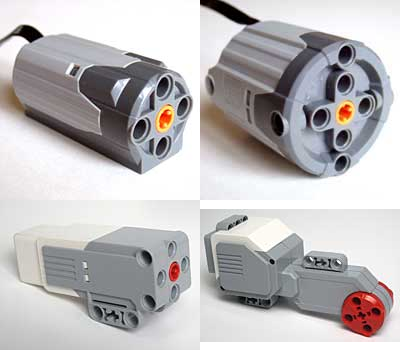
\includegraphics[width=0.6\linewidth]{images/motors}
\caption{Overview of current (2018) LEGO motors. Upper row: Power Functions large and X-large motor. Bottom row: EV3 medium and large motor}
\label{fig:motors}
\end{figure}


\subsubsection*{Power Functions Motors}
The ``Power Functions'' line of motors is designed to work with a battery pack and is intended to be controlled either with a physical switch on the battery pack or a remote control. Adapters for the power cables are required to use them in combination with the EV3 platform. \cite{power_fun}

By changing the current and polarity of the DC power supply, these motors can spin in both directions and different speeds. Because `Power Functions'' motors do not measure rotation or angle, robots utilizing them often require other means of measuring mechanical movements. Compared to the EV3 motors, they offer similar torque and mechanical power, have faster reaction speeds but offer no feedback. \cite{motor_comparison}


\subsubsection*{EV3 Servo Motors}
The EV3 robot kit contains a medium and two large servo motors. The EV3 motors use tacho feedback to measure their alignment and rotation, which allows for more precise control compared to ``Power Functions'' motors. \cite{Servo_Motor}. In strength and speed they are comparable to their ``Power Functions'' counterparts. The large EV3 motor is roughly twice as powerful as the medium one, and comes in a bigger case with different mounting points. Detailed comparisons of the mechanical and electrical properties of all LEGO motors is available at \cite{motor_comparison}.

The ev3dev programming environment offers functions for low level interactions with the EV3 motors. Available are methods to start and stop the motor, reading the angle, setting the speed and 3 different stopping patterns (coast, brake and hold). The medium and large EV3 Motor offer identical programming interfaces. For angle measurements, the motor saves the rotation at system start as 0 degrees. During operation, the current rotation angle offset to the starting point can be read by the motor. \cite{ev3_python}

\subsection*{Motor Accuracy}
Training reinforcement learning algorithms requires repetition of the same motions many times. To assume a non-adversarial environment and ensure reproduce-ability of the results, actions taken by the motors need to be accurate and consistent. We design an experiment to measure the accuracy of the motors after a series of repeated actions.

\subsubsection*{Experimental Setup}
The experiment consists of an arm attached to a motor. We rotate the arm in a 90 degree angle back and forth. After every 25 iterations we measure the offset from the starting position externally with a set square. To measure the influence of weight on the results we use two independent arms, one without a weight and the other one weighted by three heavy metals balls. The experimental set-up is shown in figure \ref{fig:angle_experiment}.

\begin{figure}
\centering
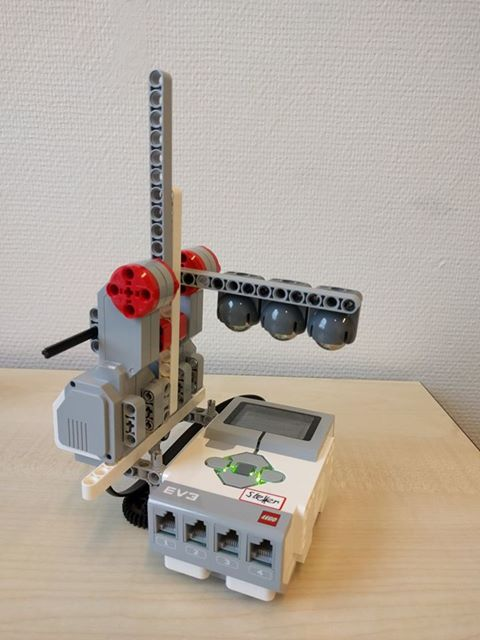
\includegraphics[width=0.35\linewidth]{images/angle_experiment}
\caption{Experiment to measure motor accuracy. The two arms (gray) swing back and forth in a 90 degree angle. One arm is weighted down by three heavy metal balls.}
\label{fig:angle_experiment}
\end{figure}



The ev3dev python bindings offer two different movement patterns: \texttt{'on\_for\_degrees()'}, which rotates the motor relative to the current position, and \texttt{'move\_to\_pos()'}, which rotates the motors to an absolute value.  Further, three stopping patterns exists: \texttt{'brake'}, \texttt{'hold'} and \texttt{'coast'}. In the experiment we will test different combinations of movement and holding patterns, to determine the configuration with the highest amount of accuracy and reproducibility. Since we want high accuracy, we do not test the coasting setting. 


\begin{table}[H]
	\centering
	\begin{tabular}{|l|l|l|l|l|l|l|}
		\hline
		Move Pattern & Stop Pattern & Weight & offset after 25 iterations & after 50it & after 75it             & after 100it            \\ \hline \hline
		relational   & hold         & no     & 1             & 1    & 2                & 2                \\ \hline
		relational   & hold         & yes    & 9             & 11   & 35               & 45               \\ \hline
		relational   & brake        & no     & 1             & 1    & 1                & 2                \\ \hline
		relational   & brake        & yes    & 35            & 50   & \textgreater{}50 & \textgreater{}50 \\ \hline
		absolute     & hold         & no     & 0             & 1    & 2                & 1                \\ \hline
		absolute     & hold         & yes    & 2             & 1    & 4                & 3                \\ \hline
		absolute     & brake        & no     & 1             & 2    & 2                & 3                \\ \hline
		absolute     & brake        & yes    & 4             & 6    & 5                & 4                \\ \hline
	\end{tabular}
	\caption{Experimental result. Angle offset in degrees after 25, 50, 75 and 100 iterations for different configurations.}
	\label{tab:angle_experiment}
\end{table}


\subsubsection*{Results}
The angle offsets measured after 25, 50, 75 and 100 iterations for different motor control settings and configurations are shown in table \ref{fig:angle_experiment}. As we can see, the non-weighted arm is very accurate in all scenarios. The results for the weighted arm differ drastically between configurations. We can observe two trends:
\begin{enumerate}
	\item The \texttt{'brake'} stopping pattern creates more offset than the \texttt{'hold'} pattern. Further observations of the experiment let us conclude that \texttt{'brake'} stops the motion of the motor, but does not block the motor for further movement after the initial momentum has been eliminated. This leads to the weighted arm pulling slightly further down between the breaking phase and the next swing of the arm. The \texttt{'hold'} stop motion holds the arm in place even after the initial momentum is eliminated. It leads to more accurate results under load.
	\item Movements ot absolute positions are more precise than relative movements. While inaccuracies of relative movements accumulate over time, movements to absolute positions only carry the inaccuracy of the last movement.
\end{enumerate}
During the experiment we also measured the range of motion that is possible without receiving any push-back from the motors. This amount of slack is consistently measured at about 12 degrees. No configuration lowered this inaccuracy. If it causes a problem later on, mechanical solutions such as a worm gear could be used to reduce the slack.

\bigskip
In conclusion, to attain the highest level of accuracy and reproducibility, motors should be moved to absolute positions and the stop pattern \texttt{'hold'} should be used. We note however that motors still allow for free movement of about 12 degrees without providing any breaking or pushback.




\subsection{Gyroscope accuracy}

\subsection{The Ultrasound Sensor}
Steffen
\subsection{The Colour Sensor}
Asger

\subsection{Need for calibration}
- most sensors no calibration
- motors and gyroscope have their 0-rotation initialized at system start. This makes reclibration nessesary every time the system is restarted. The robots should be designed with this in mind. For motors, automatic calibration can be achieved by having them hit against a push sensor first

\subsection{General building techniques}
- as simple and robust as possible
- 

\section{Reinforcement Learning with LEGO Mindstorms}
general issues arising when working with actual robots vs simulation

\section{Colour Detection}
Asger
\subsection{Problem}
what task solved
\subsection{The Robot}
description of the robot build
\subsection{The Learning}
implementation of learning, choices made in picking and implementing algorithm
\subsection{Results}
final results
\subsection{Discussion}
includes issues / future work

\section{Crawl-Robot}
Steffen
\subsection{Problem}
what task solved
\subsection{The Robot}
description of the robot build
\subsection{The Learning}
implementation of learning, choices made in picking and implementing algorithm
\subsection{Results}
final results
\subsection{Discussion}
includes issues / future work

\section{Swing-Robot}

\subsection{Problem}
what task solved
\subsection{The Robot}
description of the robot build
\subsection{The Learning}
implementation of learning, choices made in picking and implementing algorithm
\subsection{Results}
final results
\subsection{Discussion}
includes issues / future work

\section{Future Work}
Shared/independant
future robots/  multi actor learning

\section{Individual contributions}


\bibliographystyle{abbrv}
\bibliography{references}

\end{document}
